\nofiles
\documentclass[crop,tikz]{standalone}
\usepackage{amsmath}
\usepackage{amssymb}
\usepackage{tikz}
\usepackage{tikz-cd}
\usepackage{xcolor}

\usetikzlibrary{patterns, patterns.meta}
\begin{document}
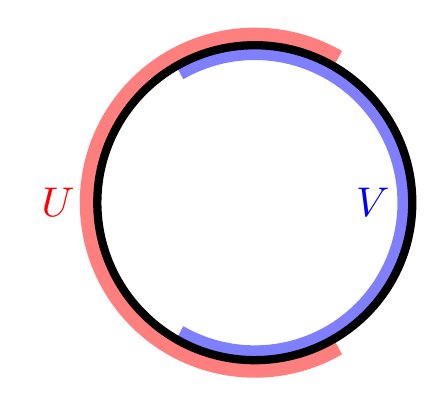
\begin{tikzpicture}
  \draw [red, line width=7,opacity=0.5,samples=100,domain=60:300] plot ({2.1*cos(\x)}, {2.1*sin(\x)});
  \draw [blue, line width=5,opacity=0.5,samples=100, domain=-120:120] plot ({1.9*cos(\x)}, {1.9*sin(\x)});
  \draw [line width=3, opacity=1] (0, 0) circle [radius=2];

  \node[scale=1.5] at (-2.5, 0) {$\color{red} U$};
  \node[scale=1.5] at (1.5, 0) {$\color{blue} V$};

\end{tikzpicture}
\end{document}